\documentclass{tufte-book}
\usepackage[utf8]{inputenc}
\usepackage[english]{babel}
\usepackage{amsmath,amsthm,amssymb}
\usepackage{tikz}
\usepackage{graphicx}
\graphicspath{{../images/}}

\setlength{\parindent}{0pt}

\title{Economics \& Project Management}
\author{Richard Robinson}

\begin{document}
\frontmatter
\maketitle
%\tableofcontents

\setlength{\parindent}{0pt}

\mainmatter


%%%%%%%%%%%%%%%%%%%%%%%%%%%%%%%%%%%%%%%%%%%%%%%%%%%%%%%%%%%%%%%%%%%%%%
% MAIN DOCUMENT
%%%%%%%%%%%%%%%%%%%%%%%%%%%%%%%%%%%%%%%%%%%%%%%%%%%%%%%%%%%%%%%%%%%%%%

\chapter{Time Value of Money}

\section{Interest Rates}

\textsc{The dimension} for an interest rate $i$ is $c_1/c_2/T$ where $c$ is a currency and $T$ is the interest period. If an amount $P$ is borrowed for $N$ periods at $i$, the final amount is \begin{equation}
  F = P(1+i)^N = P(1+i_s)^m = P + I_c
\end{equation}
which is known as compounding where the total interest on such loan $I_c$ is the compound interest. Consequently, the simple interest $I_s = PiN$ is such interest not compounded.

\bigskip
\marginnote{For example, a NIR of $i$ / year compounded monthly is $i/12$ per month.}
The \textit{nominal interest rate} (NIR) is the conventional annual interest rate. Suppose a period is divided by $m$. If $r$ is the NIR for the full period, the interest rate is
\begin{equation}
  i_s = r/m \iff r = i_s m
\end{equation}
The \textit{effective interest rate} is the actual interest rate given by \begin{equation}
  i_e = \frac{F}{P} - 1 = \left( 1 + \frac{r}{m} \right)^m - 1 \;\sim e^r - 1
\end{equation}
%
\begin{marginfigure}
  \begin{center}
    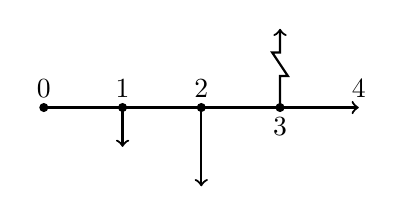
\begin{tikzpicture}
      \draw [->,thick] (0,0) -- (4,0);
      \draw [fill] (0,0) circle [radius=0.05];
      \draw [fill] (1,0) circle [radius=0.05];
      \draw [fill] (2,0) circle [radius=0.05];
      \draw [fill] (3,0) circle [radius=0.05];
      \draw [->, thick] (1,0) -- (1,-0.5);
      \draw [->, thick] (2,0) -- (2,-1);
      \draw [->, thick] (3,0) -- (3,0.4) -- (3.1,0.4) -- (2.9,0.7) -- (3,0.7) -- (3,1);
      \node [above] at (0,0) {0};
      \node [above] at (1,0) {1};
      \node [above] at (2,0) {2};
      \node [below] at (3,0) {3};
      \node [above] at (4,0) {4};
    \end{tikzpicture} \phantom{mm}
  \end{center}
  \caption{A cash flow diagram. The broken line at $t=3$ indicates the net sum of the cash flow at that period.}
\end{marginfigure}
%
A cash flow diagram is a visualization of cash flows and interest over time. Note that $N$ years from time $t$ is the end of period $N$ and beginning of $N+1$.

\section{Equivalence}




\end{document}
